
%% bare_conf.tex
%% V1.4b
%% 2015/08/26
%% by Michael Shell
%% See:
%% http://www.michaelshell.org/
%% for current contact information.
%%
%% This is a skeleton file demonstrating the use of IEEEtran.cls
%% (requires IEEEtran.cls version 1.8b or later) with an IEEE
%% conference paper.
%%
%% Support sites:
%% http://www.michaelshell.org/tex/ieeetran/
%% http://www.ctan.org/pkg/ieeetran
%% and
%% http://www.ieee.org/

%%*************************************************************************
%% Legal Notice:
%% This code is offered as-is without any warranty either expressed or
%% implied; without even the implied warranty of MERCHANTABILITY or
%% FITNESS FOR A PARTICULAR PURPOSE! 
%% User assumes all risk.
%% In no event shall the IEEE or any contributor to this code be liable for
%% any damages or losses, including, but not limited to, incidental,
%% consequential, or any other damages, resulting from the use or misuse
%% of any information contained here.
%%
%% All comments are the opinions of their respective authors and are not
%% necessarily endorsed by the IEEE.
%%
%% This work is distributed under the LaTeX Project Public License (LPPL)
%% ( http://www.latex-project.org/ ) version 1.3, and may be freely used,
%% distributed and modified. A copy of the LPPL, version 1.3, is included
%% in the base LaTeX documentation of all distributions of LaTeX released
%% 2003/12/01 or later.
%% Retain all contribution notices and credits.
%% ** Modified files should be clearly indicated as such, including  **
%% ** renaming them and changing author support contact information. **
%%*************************************************************************


% *** Authors should verify (and, if needed, correct) their LaTeX system  ***
% *** with the testflow diagnostic prior to trusting their LaTeX platform ***
% *** with production work. The IEEE's font choices and paper sizes can   ***
% *** trigger bugs that do not appear when using other class files.       ***                          ***
% The testflow support page is at:
% http://www.michaelshell.org/tex/testflow/



\documentclass[conference]{IEEEtran}
% Some Computer Society conferences also require the compsoc mode option,
% but others use the standard conference format.
%
% If IEEEtran.cls has not been installed into the LaTeX system files,
% manually specify the path to it like:
% \documentclass[conference]{../sty/IEEEtran}





% Some very useful LaTeX packages include:
% (uncomment the ones you want to load)


% *** MISC UTILITY PACKAGES ***
%
%\usepackage{ifpdf}
% Heiko Oberdiek's ifpdf.sty is very useful if you need conditional
% compilation based on whether the output is pdf or dvi.
% usage:
% \ifpdf
%   % pdf code
% \else
%   % dvi code
% \fi
% The latest version of ifpdf.sty can be obtained from:
% http://www.ctan.org/pkg/ifpdf
% Also, note that IEEEtran.cls V1.7 and later provides a builtin
% \ifCLASSINFOpdf conditional that works the same way.
% When switching from latex to pdflatex and vice-versa, the compiler may
% have to be run twice to clear warning/error messages.
\usepackage{algorithm}
\usepackage{algpseudocode} 
\usepackage{subcaption}


% *** CITATION PACKAGES ***
%
%% Use biber instead of BibTeX
%\usepackage[citestyle=numeric,style=numeric,backend=biber]{biblatex}
\usepackage[
	hyperref=true,
	%citestyle=alphabetic,
	citestyle=numeric,
	%style=alphabetic,
	style=numeric,
	sorting=none,
	maxcitenames=3,
	maxbibnames=100,
	%backref=true,
	backend=biber
]{biblatex}
\usepackage[babel,german=quotes,english=american]{csquotes} 

% disable unimportant stuff in bibliography
\DeclareSourcemap{
  \maps[datatype=bibtex, overwrite]{
    \map{
      \step[fieldset=language, null]
      \step[fieldset=notes, null]
      \step[fieldset=issn, null]
      \step[fieldset=doi, null]
      \step[fieldset=url, null]
      \step[fieldset=eprint, null]
      \step[fieldset=abstract, null]
      \step[fieldset=pages, null]
      \step[fieldset=address, null]
      \step[fieldset=editors, null]
    }
  }
}

%TODO check 
%\appto{\bibsetup}{\raggedright}
\appto{\bibsetup}{\sloppy}
\addbibresource{paper.bib}

%\DefineBibliographyStrings{english}{%
%    backrefpage  = {see p.}, % for single page number
%    backrefpages = {see pp.} % for multiple page numbers
%}




% *** GRAPHICS RELATED PACKAGES ***
%
\ifCLASSINFOpdf
\usepackage[pdftex]{graphicx}
% declare the path(s) where your graphic files are
% \graphicspath{{../pdf/}{../jpeg/}}
% and their extensions so you won't have to specify these with
% every instance of \includegraphics
% \DeclareGraphicsExtensions{.pdf,.jpeg,.png}
\else
% or other class option (dvipsone, dvipdf, if not using dvips). graphicx
% will default to the driver specified in the system graphics.cfg if no
% driver is specified.
% \usepackage[dvips]{graphicx}
% declare the path(s) where your graphic files are
% \graphicspath{{../eps/}}
% and their extensions so you won't have to specify these with
% every instance of \includegraphics
% \DeclareGraphicsExtensions{.eps}
\fi
% graphicx was written by David Carlisle and Sebastian Rahtz. It is
% required if you want graphics, photos, etc. graphicx.sty is already
% installed on most LaTeX systems. The latest version and documentation
% can be obtained at: 
% http://www.ctan.org/pkg/graphicx
% Another good source of documentation is "Using Imported Graphics in
% LaTeX2e" by Keith Reckdahl which can be found at:
% http://www.ctan.org/pkg/epslatex
%
% latex, and pdflatex in dvi mode, support graphics in encapsulated
% postscript (.eps) format. pdflatex in pdf mode supports graphics
% in .pdf, .jpeg, .png and .mps (metapost) formats. Users should ensure
% that all non-photo figures use a vector format (.eps, .pdf, .mps) and
% not a bitmapped formats (.jpeg, .png). The IEEE frowns on bitmapped formats
% which can result in "jaggedy"/blurry rendering of lines and letters as
% well as large increases in file sizes.
%
% You can find documentation about the pdfTeX application at:
% http://www.tug.org/applications/pdftex





% *** MATH PACKAGES ***
%
\usepackage{amsmath}
\usepackage{mathabx}
% A popular package from the American Mathematical Society that provides
% many useful and powerful commands for dealing with mathematics.
%
% Note that the amsmath package sets \interdisplaylinepenalty to 10000
% thus preventing page breaks from occurring within multiline equations. Use:
%\interdisplaylinepenalty=2500
% after loading amsmath to restore such page breaks as IEEEtran.cls normally
% does. amsmath.sty is already installed on most LaTeX systems. The latest
% version and documentation can be obtained at:
% http://www.ctan.org/pkg/amsmath





% *** SPECIALIZED LIST PACKAGES ***
%
%\usepackage{algorithmic}
% algorithmic.sty was written by Peter Williams and Rogerio Brito.
% This package provides an algorithmic environment fo describing algorithms.
% You can use the algorithmic environment in-text or within a figure
% environment to provide for a floating algorithm. Do NOT use the algorithm
% floating environment provided by algorithm.sty (by the same authors) or
% algorithm2e.sty (by Christophe Fiorio) as the IEEE does not use dedicated
% algorithm float types and packages that provide these will not provide
% correct IEEE style captions. The latest version and documentation of
% algorithmic.sty can be obtained at:
% http://www.ctan.org/pkg/algorithms
% Also of interest may be the (relatively newer and more customizable)
% algorithmicx.sty package by Szasz Janos:
% http://www.ctan.org/pkg/algorithmicx




% *** ALIGNMENT PACKAGES ***
%
%\usepackage{array}
% Frank Mittelbach's and David Carlisle's array.sty patches and improves
% the standard LaTeX2e array and tabular environments to provide better
% appearance and additional user controls. As the default LaTeX2e table
% generation code is lacking to the point of almost being broken with
% respect to the quality of the end results, all users are strongly
% advised to use an enhanced (at the very least that provided by array.sty)
% set of table tools. array.sty is already installed on most systems. The
% latest version and documentation can be obtained at:
% http://www.ctan.org/pkg/array


% IEEEtran contains the IEEEeqnarray family of commands that can be used to
% generate multiline equations as well as matrices, tables, etc., of high
% quality.




% *** SUBFIGURE PACKAGES ***
%\ifCLASSOPTIONcompsoc
%  \usepackage[caption=false,font=normalsize,labelfont=sf,textfont=sf]{subfig}
%\else
%  \usepackage[caption=false,font=footnotesize]{subfig}
%\fi
% subfig.sty, written by Steven Douglas Cochran, is the modern replacement
% for subfigure.sty, the latter of which is no longer maintained and is
% incompatible with some LaTeX packages including fixltx2e. However,
% subfig.sty requires and automatically loads Axel Sommerfeldt's caption.sty
% which will override IEEEtran.cls' handling of captions and this will result
% in non-IEEE style figure/table captions. To prevent this problem, be sure
% and invoke subfig.sty's "caption=false" package option (available since
% subfig.sty version 1.3, 2005/06/28) as this is will preserve IEEEtran.cls
% handling of captions.
% Note that the Computer Society format requires a larger sans serif font
% than the serif footnote size font used in traditional IEEE formatting
% and thus the need to invoke different subfig.sty package options depending
% on whether compsoc mode has been enabled.
%
% The latest version and documentation of subfig.sty can be obtained at:
% http://www.ctan.org/pkg/subfig




% *** FLOAT PACKAGES ***
%
%\usepackage{fixltx2e}
% fixltx2e, the successor to the earlier fix2col.sty, was written by
% Frank Mittelbach and David Carlisle. This package corrects a few problems
% in the LaTeX2e kernel, the most notable of which is that in current
% LaTeX2e releases, the ordering of single and double column floats is not
% guaranteed to be preserved. Thus, an unpatched LaTeX2e can allow a
% single column figure to be placed prior to an earlier double column
% figure.
% Be aware that LaTeX2e kernels dated 2015 and later have fixltx2e.sty's
% corrections already built into the system in which case a warning will
% be issued if an attempt is made to load fixltx2e.sty as it is no longer
% needed.
% The latest version and documentation can be found at:
% http://www.ctan.org/pkg/fixltx2e


%\usepackage{stfloats}
% stfloats.sty was written by Sigitas Tolusis. This package gives LaTeX2e
% the ability to do double column floats at the bottom of the page as well
% as the top. (e.g., "\begin{figure*}[!b]" is not normally possible in
% LaTeX2e). It also provides a command:
%\fnbelowfloat
% to enable the placement of footnotes below bottom floats (the standard
% LaTeX2e kernel puts them above bottom floats). This is an invasive package
% which rewrites many portions of the LaTeX2e float routines. It may not work
% with other packages that modify the LaTeX2e float routines. The latest
% version and documentation can be obtained at:
% http://www.ctan.org/pkg/stfloats
% Do not use the stfloats baselinefloat ability as the IEEE does not allow
% \baselineskip to stretch. Authors submitting work to the IEEE should note
% that the IEEE rarely uses double column equations and that authors should try
% to avoid such use. Do not be tempted to use the cuted.sty or midfloat.sty
% packages (also by Sigitas Tolusis) as the IEEE does not format its papers in
% such ways.
% Do not attempt to use stfloats with fixltx2e as they are incompatible.
% Instead, use Morten Hogholm'a dblfloatfix which combines the features
% of both fixltx2e and stfloats:
%
% \usepackage{dblfloatfix}
% The latest version can be found at:
% http://www.ctan.org/pkg/dblfloatfix




% *** PDF, URL AND HYPERLINK PACKAGES ***
%
\usepackage{url}
% url.sty was written by Donald Arseneau. It provides better support for
% handling and breaking URLs. url.sty is already installed on most LaTeX
% systems. The latest version and documentation can be obtained at:
% http://www.ctan.org/pkg/url
% Basically, \url{my_url_here}.

%\usepackage{asmfonts}

% *** Do not adjust lengths that control margins, column widths, etc. ***
% *** Do not use packages that alter fonts (such as pslatex).         ***
% There should be no need to do such things with IEEEtran.cls V1.6 and later.
% (Unless specifically asked to do so by the journal or conference you plan
% to submit to, of course. )

\usepackage{pgfplots}

% correct bad hyphenation here
\hyphenation{op-tical net-works semi-conduc-tor}


\begin{document}
	%
	% paper title
	% Titles are generally capitalized except for words such as a, an, and, as,
	% at, but, by, for, in, nor, of, on, or, the, to and up, which are usually
	% not capitalized unless they are the first or last word of the title.
	% Linebreaks \\ can be used within to get better formatting as desired.
	% Do not put math or special symbols in the title.
	\title{Probabilistic Symbol Encoding for \\Convolutional Associative Memories}
	
	
	% author names and affiliations
	% use a multiple column layout for up to three different
	% affiliations
	\author{\IEEEauthorblockN{Igor Peric, Alexandru Lesi, Daniel Spies, Stefan Ulbrich, R{\"u}diger Dillman, Marius Z{\"o}llner}
		\IEEEauthorblockA{FZI Forschungszentrum Informatik\\
			Karlsruhe, Germany\\
			Email: $\{$peric, lesi, spies, ulbrich, dillmann, zoellner$\}$@fzi.de}
	}
	
	% conference papers do not typically use \thanks and this command
	% is locked out in conference mode. If really needed, such as for
	% the acknowledgment of grants, issue a \IEEEoverridecommandlockouts
	% after \documentclass
	
	% for over three affiliations, or if they all won't fit within the width
	% of the page, use this alternative format:
	% 
	%\author{\IEEEauthorblockN{Michael Shell\IEEEauthorrefmark{1},
	%Homer Simpson\IEEEauthorrefmark{2},
	%James Kirk\IEEEauthorrefmark{3}, 
	%Montgomery Scott\IEEEauthorrefmark{3} and
	%Eldon Tyrell\IEEEauthorrefmark{4}}
	%\IEEEauthorblockA{\IEEEauthorrefmark{1}School of Electrical and Computer Engineering\\
	%Georgia Institute of Technology,
	%Atlanta, Georgia 30332--0250\\ Email: see http://www.michaelshell.org/contact.html}
	%\IEEEauthorblockA{\IEEEauthorrefmark{2}Twentieth Century Fox, Springfield, USA\\
	%Email: homer@thesimpsons.com}
	%\IEEEauthorblockA{\IEEEauthorrefmark{3}Starfleet Academy, San Francisco, California 96678-2391\\
	%Telephone: (800) 555--1212, Fax: (888) 555--1212}
	%\IEEEauthorblockA{\IEEEauthorrefmark{4}Tyrell Inc., 123 Replicant Street, Los Angeles, California 90210--4321}}
	
	
	% use for special paper notices
	%\IEEEspecialpapernotice{(Invited Paper)}
	
	
	% make the title area
	\maketitle
	
	% As a general rule, do not put math, special symbols or citations
	% in the abstract
	\begin{abstract}
		Vector Symbolic Architectures (VSAs) define a set of operations
		for association, (compressed) storage, manipulation and retrieval
		of symbolic concepts, represented as fixed-length vectors in
		${\rm I\!R}^n$.
		A specific instance of VSAs, Holographic Reduced Representations (HRRs),
		have proven to exhibit properties similar to human short-term
		memory and are, as such, interesting for computational modeling.
		In this paper we extend the HRR approach by introducing implicit,
		topology-preserving encoding and decoding procedures.
		We propose moving away from traditional exact symbolic representation
		to probabilistic one, replacing unique symbol identifiers with 
		probability density function.
		As we discover, this requires randomly chosen permutations for encoding and
		their corresponding inverse for decoding. These are necessary
		for the uniform distribution of signals across Fourier space where
		embedding takes place.
		These novel encoding schemes, together with the extended operation
		pipeline, are eliminating the need for so-called \emph{clean-up modules} after memory
		retrieval (e.g., self-organizing maps). Effectively, encoding
		implicitly represents the scalar symbol, so no further lookup is needed.
		We show that our encoding scheme has a positive impact
		on memory capacity in comparison to the original capacity
		benchmark for HRRs by Plate
		\cite{Plate:1995:HolographicReducedRepresentations}.
		We also evaluate our memories in two different robotics tasks: visual scene memory and state machine scripting (holographic controllers).
	\end{abstract}
	
	% no keywords
	
	
	
	
	% For peer review papers, you can put extra information on the cover
	% page as needed:
	% \ifCLASSOPTIONpeerreview
	% \begin{center} \bfseries EDICS Category: 3-BBND \end{center}
	% \fi
	%
	% For peerreview papers, this IEEEtran command inserts a page break and
	% creates the second title. It will be ignored for other modes.
	\IEEEpeerreviewmaketitle
	
	
	
	\section{Introduction}
	
	Vector Symbolic Architectures (VSA) define a set of operations for storage (compression) and retrieval of symbolic concepts in fixed size vectors.
As described in \cite{Levy:2008:VectorSymbolicArchitectures}, every VSA has to implement three basic operations:
	\begin{enumerate}
		\item association (binding) $\mapsto \otimes$
		\item superposition (appending) $\mapsto +$
		\item probing (unbinding) $\mapsto \oslash$
	\end{enumerate}
	
	In addition, every VSA can be considered as a lossy compression technique, since binary operations on N-element vectors return N-element vectors as well. These operations will be described in further detail in the following section. 
	
	Depending on the way these three operations are implemented we can distinguish several popular VSAs, such as Holographic Reduced Representations \cite{Plate:1995:HolographicReducedRepresentations}, Circular HRRs \cite{DeVine:2010:Semanticoscillations}, Binary Spatter Codes \cite{Kanerva:1994:SpatterCodeEncoding}, Holographic Graph Neurons \cite{Kleyko:2016:HolographicGraphNeuron}, Geometric Algebras \cite{Patyk-Lonska:2011:DistributedRepresentationsBased} and Random Permutations \cite{Recchia:2015:EncodingSequentialInformation}.
The most widely used ones are HRRs and they are briefly explained in section \ref{sec:hrr}.
Authors in \cite{Golosio:2015:CognitiveNeuralArchitecture} have used them to solve word embedding problem for extremely large dataset by replacing computationally expensive big matrix factorization with an iterative estimation algorithm based on HRRs.
Some of the other work is centered around pattern recognition \cite{Kleyko:2016:PatternRecognitionVector} and functional large-scale cognitive architecture models \cite{Eliasmith:2012:LargeScaleModel}.
Preliminary theoretical assumptions have been made about the ability to use them as agent controllers \cite{Levy:2013:LearningBehaviorHierarchies}, where a symbolic program is represented with a set of combined symbolic actions associated with actuator symbols and symbolic sensing.
	
	
	\begin{figure}
		\center
		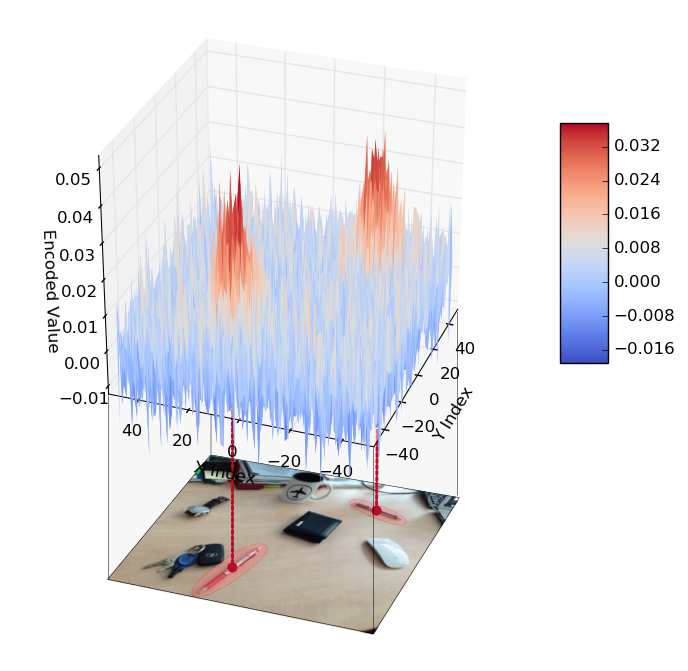
\includegraphics[width=0.9\columnwidth]{img/probe_for_pen_w_img.png}
		\caption{In-memory representation of visual scene short-term memory. The result shows probability distribution for a symbol "pen" being at certain position in scene.}
	\end{figure}
	
	
	Authors in \cite{Eliasmith:2012:LargeScaleModel} have demonstrated that the functional cognitive model Spaun is capable of performing 7 different cognitive tasks when implemented as HRRs using biologically plausible models of neuron dynamics.
They further show that in serial working memory tasks the model of forgetting exhibits similar behaviour as human working memory due to limited capacity.
Lastly they report similarity between the human working memory capacity and the average number of items (symbols) that their model is capable of holding in memory.

	This successful model of forgetting is one of the reasons our work is centred around HRRs. Another reason is the fact that HRRs are the only VSAs up to date operating on convolution operations in their core.
This is appealing if we take the numerous recent advancement in deep learning and convolutional neural networks into consideration.
These networks succeed due to training on big data and using convolution as the main architectural constraint.
Although the description of the biophysical mechanism underlying convolution and concept of weight sharing are still missing, it is important to reuse proven concepts, such as convolutional filtering, in as general way as possible.
In other words, addressing multiple fundamentally different problems with similar computational principles can be considered a step towards a unified brain processing theory.
	
	\section{Vector Symbolic Architectures}
	
In order to use VSA operations all types of required inputs need to first be represented as symbols, which are vectors of fixed size. The basic approach is to pick these vectors randomly once for each input used in any operation and maintain these pairs in a separate data structure.	
	\\
	
	\textbf{Association} (also called "binding") is the operation of linking two operands together, resulting in a vector of the same size which is dissimilar (or orthogonal) to the original vectors, but also contains scrambled information from both of them.
For instance, linking the property "red" to object "triangle" can be done using the binding operation as follows:
	
	\begin{equation}
	memory_1 = red \otimes triangle
	\end{equation}
	
	\textbf{Superposition} is the operation of extending a set of items, regardless of what is already contained in them.
As an example, a memory of "red triangle and blue circle" can be formed in the following way:
	\begin{equation}
	memory_2 = memory_1 + blue \otimes circle
	\end{equation}
	
	\textbf{Probing} is the operation of extracting a noisy version of an associated item from a joint set memory.
I.e. in this scenario the question "What color is the triangle?" could be asked like this:
	
	\begin{equation}
	red \approx memory_2 \oslash triangle
	\end{equation}
	
	
	The probing operation assumes the existence of inverse elements, so the previous equation can be interpreted and explained as such:
	\begin{multline}
	memory_2 \otimes triangle'=\\
	(red \otimes triangle + blue \otimes circle) \otimes triangle'=\\
	red \otimes triangle  \otimes triangle' + blue \otimes circle \otimes triangle' =\\
	red + blue \otimes circle \otimes triangle'  = red + noise
	\approx red
	\end{multline}
	
	Here $triangle'$ represents the inverse of $triangle$.
The resulting vector will be a composition of something that is very similar to $red$ and something that doesn't resemble anything meaningful from the symbol table, so it can be treated as negligible noise.	A usual way of computing similarity is the cosine distance, which for two vectors \pmb x and \pmb y is calculated as follows:
	
	\begin{equation}
cos(\pmb x, \pmb y) = \frac {\pmb x \cdot \pmb y}{||\pmb x|| \cdot ||\pmb y||}
	\end{equation} 
	
	Obtained values of similarity clearly distinguish the matching vectors. Concrete values that highlight this will be later presented in section \ref{sec:experiments}.	

	The process of converting the noisy result of probing into the closest known symbol is called the \textbf{clean-up procedure}.
A straightforward way of implementing clean-up memory is using a lookup table, while other researchers show that any type of attractor network can be used (e.g. self-organizing maps).

	In the case of lookup tables, in order to decode a specific symbolic vector, the elements from a symbol table are iterated over, the similarity to each of the entries is calculated and the symbol which presented maximum similarity is returned. With the help of a threshold for the similarity value false-positives can be excluded. A lookup requires $O(n)$, where $n$ is the number of symbols known to the system. This approach works quite well for object identifiers (names), but has some non-desirable properties when used on scalar encoding. The space complexity will increase and may become infeasible, depending on the number of inputs needed. One way of handling symbolic scalar encoding is to discretize the whole input range into bins and assigning a random vector to each discrete value. This however may often prove to not satisfy the task needs any more.

	
	\subsection{Holographic reduced representations}
	\label{sec:hrr}
	
	Holographic Reduced Representations are VSAs which implement the operation of binding as circular convolution. One option for calculating it is with the help of discrete Fast Fourier Transformations, in short FFTs. Taking $f(x)$ to describe an FFT, with $f^{-1}(x)$ as its inverse, circular convolution can be calculated as follows:
	
	\begin{equation}
	\pmb a = f^{-1}(f(\pmb x) * f(\pmb y))
	\end{equation}
	
	where $\pmb a$ is the result of convolution, and $\pmb x$ and $\pmb y$ are symbolic vectors of size $n$.
Superposition is implemented as a simple element-wise vector addition. Taking the result of the previously displayed convolution and superposing it with some vector $\pmb b$ is done as follows:

	\begin{equation}
	\pmb m = \pmb a + \pmb b
	\end{equation}

The resulting vector of the superposition operation $\pmb m$ can then be probed by using the inverse of circular convolution, which is circular correlation. Plainly put probing can be viewed as binding with the "inverse" of a vector in Fourier space:
	
	\begin{equation}
	\pmb y^* = f^{-1}(f(\pmb m) * f(\pmb x)^{-1})
	\end{equation} 

Following the previous formulas as a series of operations the vector $\pmb y^*$ will be similar to vector $\pmb y$, but not entirely the same due to the noisy influence of vector $\pmb b$. The inverse in Fourier space referred to here is gained by calculating the complex conjugate of the vector's entries. Complex conjugates are simply the same values with negated imaginary parts.
		
	Performing FFTs has no invariant regarding the mean of the resulting vector entries and can produce all sorts of results.
Due to this, when probing, we would receive vectors which had the correct relative distance between their values, i.e.
the correct "shape", but would be shifted, stretched or squeezed along the Y-axis. This lead to vectors falsely being regarded as dissimilar to each other, and can be solved by performing two normalization steps before comparing:

	\begin{equation}
	x_i = x_i - \frac{\sum_{i=0}^n ||x_i||}{|x|}
	\end{equation} 	
	
	\begin{equation}
	\pmb x = \frac{\pmb x }{ \| \pmb x \|}
	\end{equation} 	
	
	\section{Topology-preserving encoding}
	
	\subsection{Encoding scalar symbols}
	
	Encoding scalars is a good example for the necessity of preserving topology.
Depending on what dataset is in use it may be required to store mappings for any number of values, which can drastically increase space requirements.
Furthermore, using a separate random encoding for each scalar, regardless of whether they are very close to each other or not, there would be no similarity in neighbouring values.
For example, the following probe will yield no result:
	
	\begin{equation}
	(10000 \otimes a) \oslash 10001
	\end{equation}
	
	To facilitate these two qualities scalar encoding can be achieved with the help of radial basis functions. Among these functions one of the options are Gaussian distributions.
The encoded vector can simply represent a Gaussian sampled over a fixed input range.
Figure \ref{no-perm-a} shows how such an encoded vector looks like, and what the result of binding it to a generic random vector is.
With this result it becomes obvious that unfortunately lots of information is lost.
If this result is probed with the same random vector used in binding something similar to the initial Gaussian distribution is expected.
And yet figure \ref{no-perm-b} presents no such outcome.
While there is a peak at the initial value lots of other peaks also arise, making it impossible to detect which one is correct.

	
	\begin{figure}[th!]
		\begin{subfigure}{1\columnwidth}
			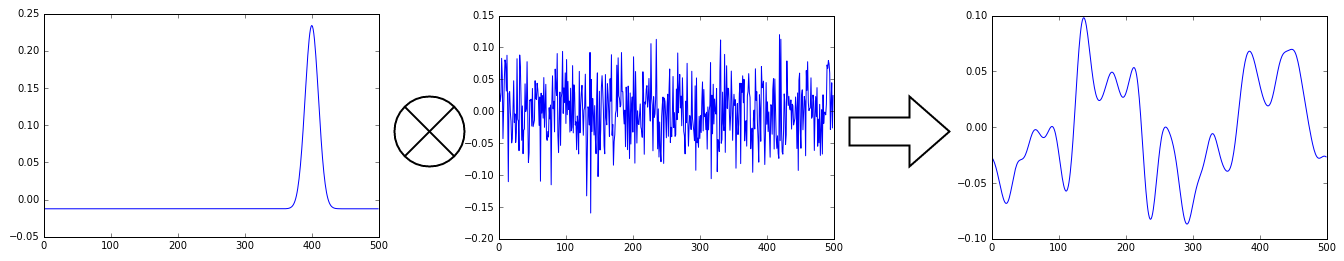
\includegraphics[width=\columnwidth]{img/scalar-pre-perm.png}
			\caption{Binding}
			\label{no-perm-a}
		\end{subfigure}
		\begin{subfigure}{1\columnwidth}
			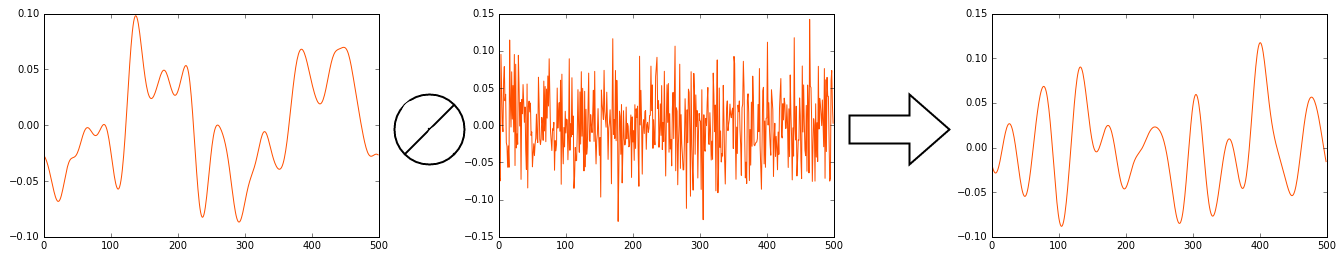
\includegraphics[width=\columnwidth]{img/scalar-pre-perm-probe.png}
			\caption{Probing}
			\label{no-perm-b}
		\end{subfigure}
		\caption{Plot of vector values.
Figure \ref{no-perm-a} shows the binding of the value 8 on a scale to 10 with the symbolic representation of "ball", which is random.
In figure \ref{no-perm-b} "ball" is being probed, and the expected result is a Gaussian distribution for 8, mixed with some noise.}
		\label{no-perm}
	\end{figure}
	
	This effect is due to the fact that circular convolution is based on Fourier transformations. A lack of frequencies in the Fourier space of the encoded scalar becomes apparent, as highlighted in figure \ref{fft}.
All the information of a Gaussian distribution is crammed into the lowest and highest values of the Fourier transformation, resulting in a high loss of information.
In these circumstances, when probing for a scalar, the vector received is in turn recreated of too few frequencies and will not come close to resembling the original Gaussian distribution.


\begin{figure}[th!]
	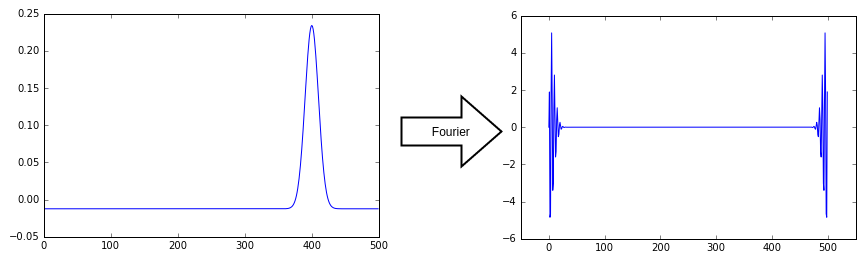
\includegraphics[width=\columnwidth]{img/scalar-pre-perm-fft.png}
	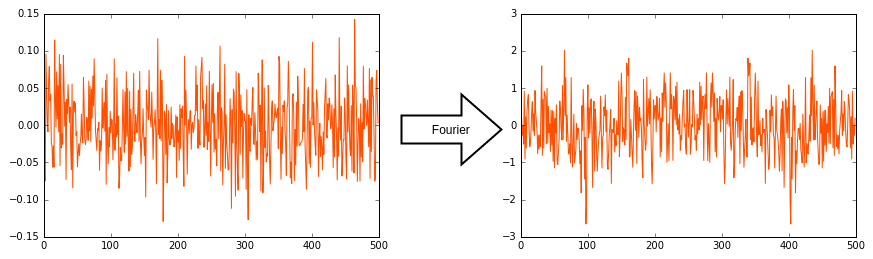
\includegraphics[width=\columnwidth]{img/scalar-random-fft.png}
	\caption{Fourier analysis of 1D symbols: a Gaussian distribution (top row) and a randomly sampled vector of the same size (bottom row). It is obvious that the latter's information in Fourier space is uniformly spread across the whole spectrum, while the former's is concentrated around 2 boundary points.}
	\label{fft}
\end{figure}
	
	This inconvenience is removed with the help of permutations.
Depending on the size of the memory vectors used a fixed permutation is generated once.
Whenever a scalar is encoded the Gaussian distribution is first sampled over the given range, after which the sampled values swap places accordingly.
As such the resulting vector will present lots of jumps in value, which have a significant impact on the Fourier space, as can be seen in figure \ref{perm-fft}.
	
	\begin{figure}
		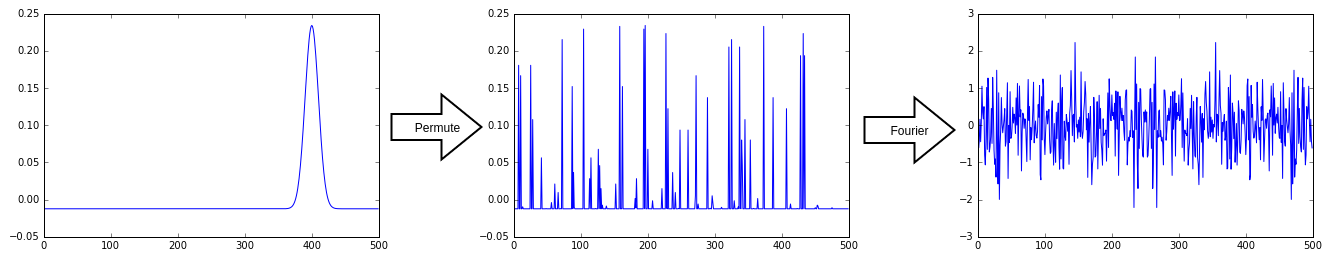
\includegraphics[width=\columnwidth]{img/scalar-perm-step-fft.png}
		\caption{Applying random permutation to a sampled Gaussian distribution results in more discrete changes in signal, which correspond to high-frequency components in Fourier space. This makes frequency spectrum spread more uniform, which is a desirable property for HRRs. Although this scrambling of initial signal makes it seem random, the fact that the same permutation is used in all encodings keeps two semantically close values having very similar representations, thus preserving their semantic proximity. }
		\label{perm-fft}
	\end{figure}
	
	Working with such a vector makes it possible to successfully probe for scalars and receive a Gaussian distribution overlapped with some noise.
All of this can be seen in figure \ref{perm}, which depicts the exact same operations as figure \ref{no-perm}, but using a permuted version of a Gaussian distribution.
The result in figure \ref{perm-b} clearly shows a spike at the expected spot in the sample range.
This vector can now be smoothed out, after which the peak can easily be identified and the initial scalar can be recovered.
	
	\begin{figure}
		\begin{subfigure}{1\columnwidth}
			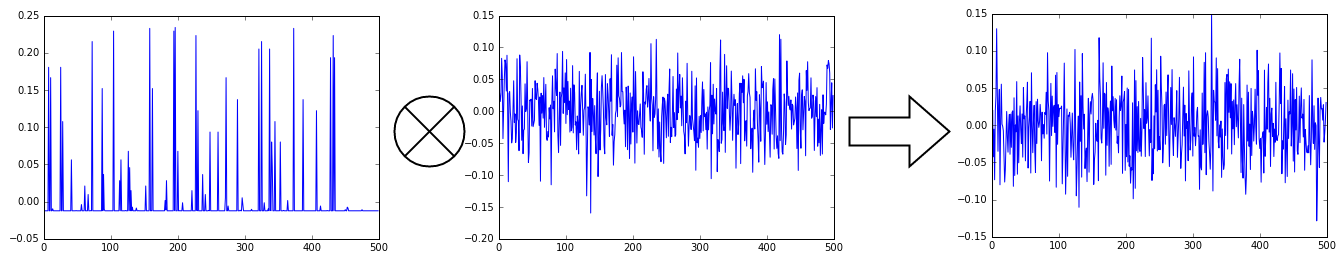
\includegraphics[width=\columnwidth]{img/scalar-post-perm.png}
			\caption{Binding}
			\label{perm-a}
		\end{subfigure}
		\begin{subfigure}{1\columnwidth}
			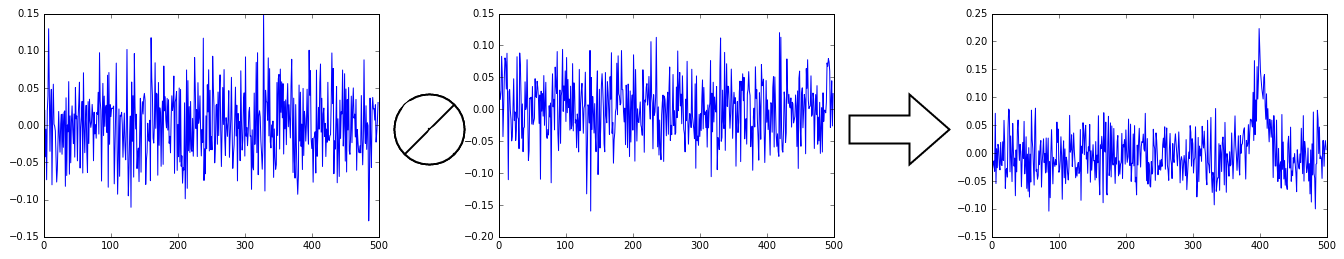
\includegraphics[width=\columnwidth]{img/scalar-post-perm-probe.png}
			\caption{Probing}
			\label{perm-b}
		\end{subfigure}
		\caption{Figure \ref{perm-a} shows the binding of the permuted Gaussian distribution for the value 8 from range [1, 10] with the symbolic representation of "ball", which is random.
In figure \ref{perm-b} "ball" is being probed, and the result after inverse permutation is a Gaussian distribution for the value 8, mixed with some noise.}
		\label{perm}
	\end{figure}
	
	Algorithms 1 and 2 show the operations pipeline before and after the suggested modification are introduced in pseudo code.
	
	\begin{algorithm}
		\caption{Original pipeline}
		\begin{algorithmic}[1]
			\ForAll{$symbol$}
			\State $t_{symbol} \gets chooseRandomVector()$
			\EndFor
			\State $m \gets initEmptyMemory()$
			\ForAll{$(symbol_1, symbol_2)$}
			\State $enc_1 \gets FFT(t_{symbol_1})$
			\State $enc_2 \gets FFT(t_{symbol_2})$
			\State $m \gets m + IFFT(enc_1 * enc_2$)
			\EndFor		
			\Function{ProbeMemory}{memory, op}
			\State $result\gets IFFT(FFT(memory)* FFT(op)^{-1})$
			
			\ForAll{$symbol$}
			\State $s \gets cosineSimilarity(t_{symbol}, result)$
			\If {$s \geq cleanResultSimilarity$}
			\State $cleanResultSimilarity \gets s$
			\State $cleanResult \gets t_{symbol}$
			\EndIf
			\EndFor \\
			\Return $cleanResult$
			\EndFunction
		\end{algorithmic}
	\end{algorithm}
	
	
	Lines 1-3 assign a random vector representation to each symbol known to the system prior to any other operations. This lookup table is stored in an array $t$. Lines 4-9 initialize the memory $m$ with an arbitrary amount of pairs of associated scalars. Function $ProbeMemory(memory, op)$ returns a symbol associated with provided $op$. Line 11 performs circular correlation and stores the noisy result of unbinding in $s$. Lines 12-18 loop through the whole lookup table and find the maximum similarity vector to $s$.
		
		\begin{algorithm}
			\caption{Modified pipeline}
			\begin{algorithmic}[1]
				\State $P \gets chooseRandomPermutation(n)$
				\State $m \gets initEmptyMemory()$
				\ForAll{$(symbol_1, symbol_2)$}
				\State $enc_1 \gets FFT(permute(enc(symbol_1, n), P))$
				\State $enc_2 \gets FFT(permute(enc(symbol_2, n), P))$
				\State $m \gets m + IFFT(enc_1 * enc_2)$
				\EndFor	
				\Function{ProbeMemory}{memory, op}
				\State $r \gets IFFT(FFT(memory) * FFT(op)^{-1})$
				\State $r \gets permute(r, P^{-1})$
				\State $cleanResult \gets argmax(r)$
				
				\Return $cleanResult$
				\EndFunction
			\end{algorithmic}
		\end{algorithm}
		
		In contrast, Algorithm 2 shows a pipeline with our proposed changes. The first line chooses a fixed random permutation of $n$ elements used throughout the whole process. There is no initial loop to assign symbolic representations to all symbols. They are, instead, constructed according to need using function $enc(value, n)$. This function returns a discrete sampled Gaussian distribution vector of $n$ elements, centred around a chosen $value$. The vector is then permuted using a permutation $P$ in lines 4 and 5, so its frequency representation contains uniform spread over the whole spectrum, as explained earlier in this chapter. The probing operation consists of applying an inverse permutation $P^{-1}$ after IFFT (line 10). Since this returns a noisy version of the initial Gaussian distribution (shown in figure \ref{perm-b}), the only thing that needs to be done is to identify the peak of the distribution. The complexity of this operation is linear w.r.t. length of the vector $n$, while in the case of Algorithm 1 it is linear w.r.t. to number of symbols stored in the lookup table.
		

	\subsection{Encoding coordinate symbols}
			
		Encoding coordinate symbols works in a manner very similar to encoding scalar symbols. Depending on the number of coordinates the symbolic vectors shape is reinterpreted. 2D coordinates, for instance, require a matrix. This matrix represents the entire coordinate space and on it 2D Gaussian distributions are sampled. It can be viewed as a heat map, as displayed in figure \ref{fig:encoding-coord}.	The matrix will still be treated as a vector when it comes to running operations on it and must also be permuted. Since the value space now has more dimensions the size of the vector has to be raised accordingly to achieve performance similar to that of scalar symbol encoding. 
		
		An attempt has been made to overcome the curse of dimensionality by splitting the vector up in the number of dimensions and simply encoding the value for each dimension in the resulting sub-vectors. Unfortunately it then becomes impossible to differentiate among multiple coordinates encoded in the same vector. Specifically, when decoding, there is no way to know which of the values in separate sub-vectors belong to each other and which don't. On the other hand if only a single coordinate needs to be bound to another symbol this approach is still feasible and will permit the use of smaller vectors for high accuracy. Concretely, for $d$ dimensions, splitting up the vector will require the size to be raised by a factor of $d$ to maintain the same accuracy. Reinterpreting the shape will require the size to increase exponentially by the power of $d$ to keep the accuracy.
			
	\section{Properties of holographic memories}
	
	Vector Symbolic Architectures in general have the following properties:
	\begin{itemize}
		\item The number of items stored in a single memory vector is not known based solely on it's content.
		\item Existence of an item in memory cannot be checked explicitly. The closest equivalent is to probe the memory for the item of interest and to compare the similarity of the decoded result to anything meaningful. Even then it could be that the result of probing for anything might still require to be probed by a further symbol to retrieve the sought out item.
		\item Chances of successful recall depend on the actual stored data.
		\item Memories can be changed in an online fashion. There is no need to recreate memories from scratch - symbols can be appended to or removed from already existing memory vectors if present.
	\end{itemize}
	
		\begin{figure}[th!]
			\begin{subfigure}{0.45\columnwidth}
				\center
				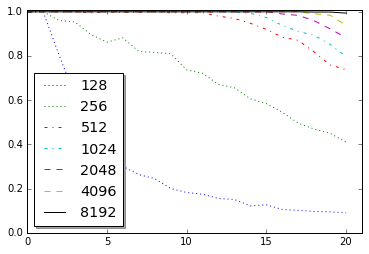
\includegraphics[width=1\columnwidth]{img/capacity.png}
				\caption{Binding pairs of random vectors. Accuracy decreases with more bindings.}
				\label{fig:capacity}
			\end{subfigure}
			\begin{subfigure}{0.45\columnwidth}
				\center
				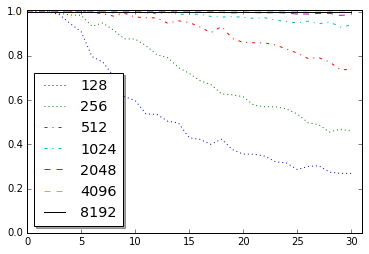
\includegraphics[width=1\columnwidth]{img/capacity_scalar_30.png}
				\caption{Binding pairs of one scalar and a random symbol, then probing for the scalar.}
				\label{fig:capacity_scalar}
			\end{subfigure}	
			\center
			\begin{subfigure}{0.45\columnwidth}
				\center
				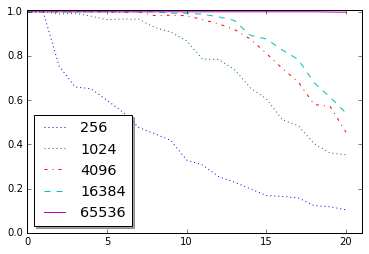
\includegraphics[width=1\columnwidth]{img/capacity_coordinate.png}
				\caption{Binding pairs of one 2D coordinate and a random symbol, then probing for the scalar.}
				\label{fig:capacity_coordinate}
			\end{subfigure}	
			\caption{Memory capacity analysis for storing a variable number of pair associations in a single memory vector. Different lines show various vector lengths, the horizontal axis shows the number of pairs and vertical axis accuracy of successful recall. Both false positives and false negatives are regarded.}
		\end{figure}	
	
	
	\subsection{Capacity}
	
	Just as Plate has done in the original HRR paper \cite{Plate:1995:HolographicReducedRepresentations} we have tested the memory capacity in terms of accuracy of successful recall for variable numbers of bound pairs. Results are shown in figure \ref{fig:capacity}.
	
	As we can see, a 512 element vector starts decreasing accuracy of recall after 10 pairs stored in a single memory block. A 4096 and 8192 element vectors can almost perfectly recall 20 associated pairs, which matches the results of Plate using a lookup table and a clean-up process. 
	
	The experiment was repeated for binding a random symbol to the encodings of both scalars and to 2D coordinates, to compare performance. Figure \ref{fig:capacity_scalar} shows the result for scalars. In this instance the probe was always done for the scalar value. The total accuracy of the result depends on new factors, the main of which will be the quality of the smoothing function used to clean up the noise from the resulting signal. This will determine how much the peaks position may shift in some direction. In our experiments a Hanning window smoothing technique was used and a 2\% deviance from the exact initial scalar was allowed. With these settings probing performed significantly better than solely among random symbols. Vectors of size 8192 even managed to maintain 100\% accuracy when storing 30 bindings. Intuitively this can be explained as follows: Gaussian distributions are far more noise tolerant than random vectors. Vectors need to maintain a high similarity to be declared identical, whereas Gaussian distributions only need to present peaks after smoothing. 
	
	Finally figure \ref{fig:capacity_coordinate} shows the accuracy of stacking bindings of 2D coordinates with random symbols. The same smoothing and deviance settings were used as for the previous experiment. As coordinates are encoded in a vector that is virtually cast to 2D its length would have to be squared to achieve similar performance to scalars. Due to this higher steps in between vector lengths have been used, and most lengths still perform rather poorly. However, increasing the length considerably, like in the case with 65536 elements, near-perfect accuracy can still be upheld up to 20 bindings.
		

		
	\section{Experiments}
	\label{sec:experiments}
	\subsection{Visual short term memory and top-down attention model}
	
	In this experiment a system is given a monocular stream as an input. An arbitrary algorithm is used to perform object detection and recognition, resulting in a number of 2D coordinates associated with respective object names (figure \ref{fig:object-detection}). Object names are strings and are encoded as random vectors of length $n$, which are sampled from a Gaussian distribution (figure \ref{fig:encoding-object}). The locations of objects in the image plane are 2D coordinates $(x,y)$ and they are perceptually grounded symbols (figure \ref{fig:encoding-coord}).

	
	\begin{figure}[th!]
		\center
		\begin{subfigure}{1.0\columnwidth}
			\center
			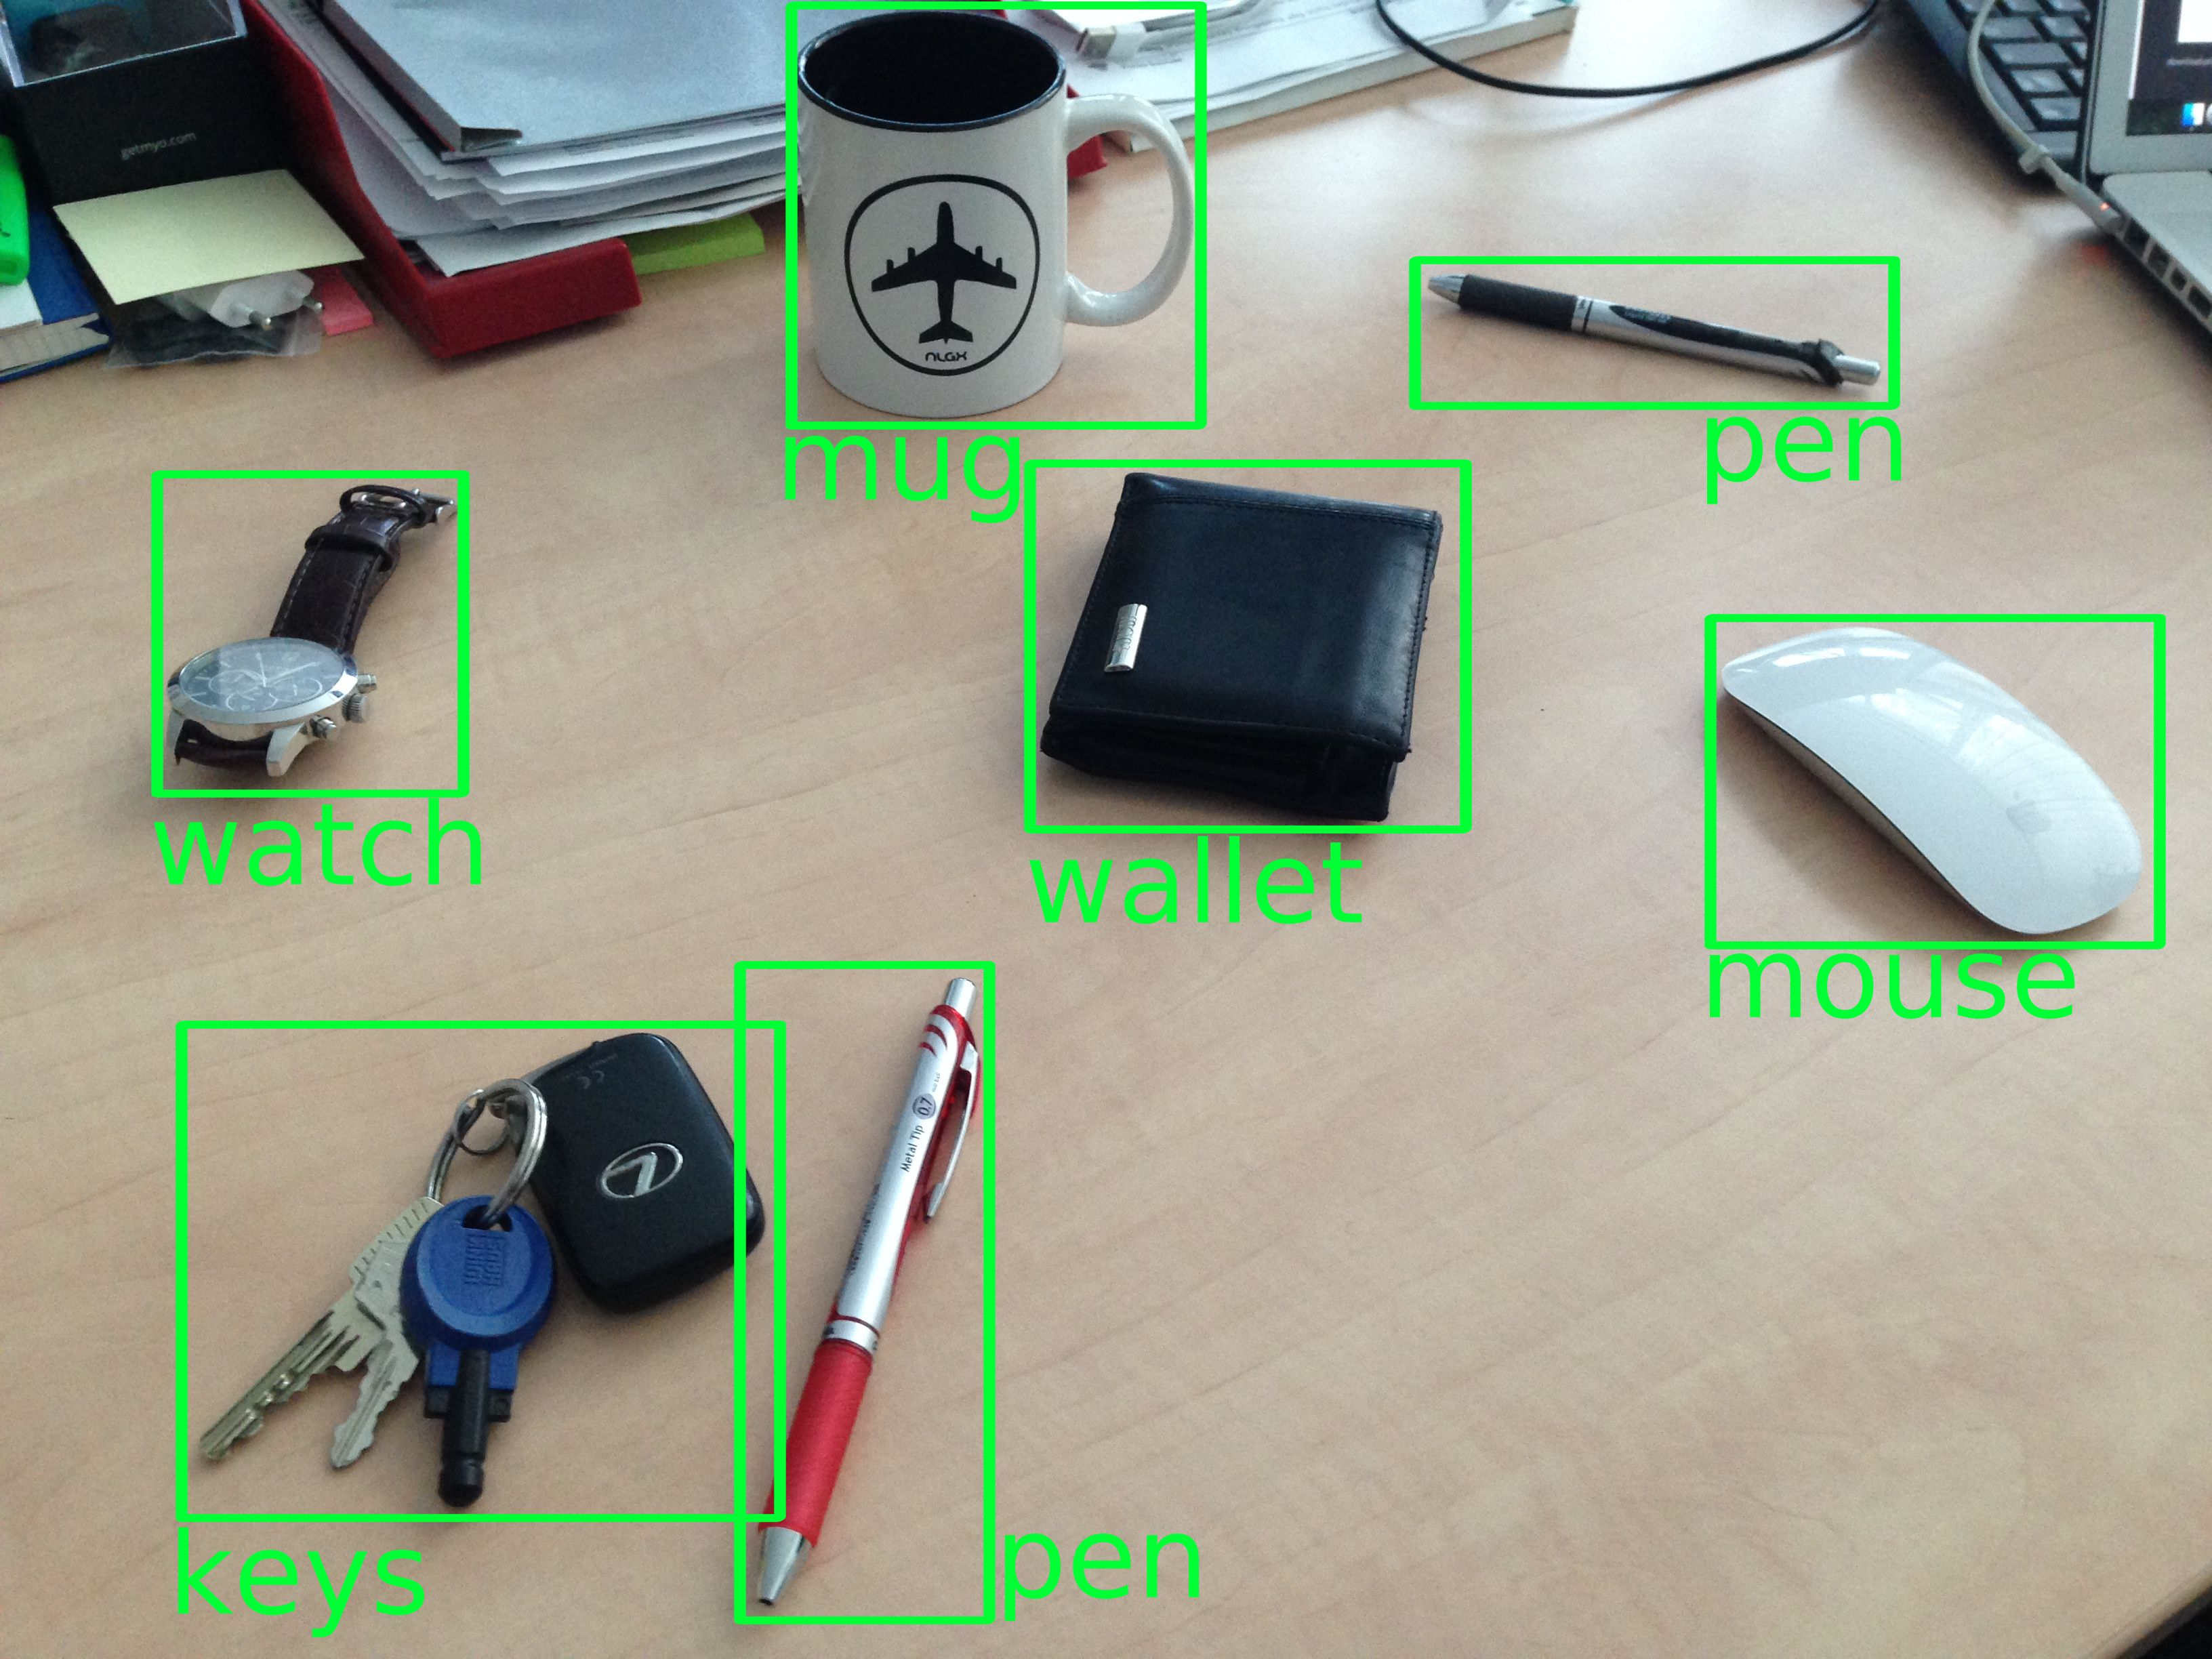
\includegraphics[width=0.6\columnwidth]{img/map_original.jpg}
			\caption{Original scene and a set of detected objects}
			\label{fig:object-detection}
		\end{subfigure}
		
		\begin{subfigure}{0.45\columnwidth}
			\center
			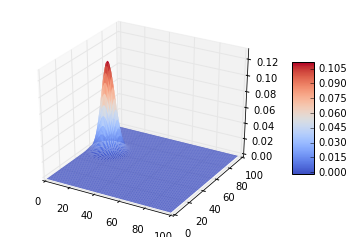
\includegraphics[width=\linewidth]{img/coord_example_1.png}
			\caption{Encoding of location (x,y) for "watch"}
			\label{fig:encoding-coord}
		\end{subfigure}
		\begin{subfigure}{0.45\columnwidth}
			\center
			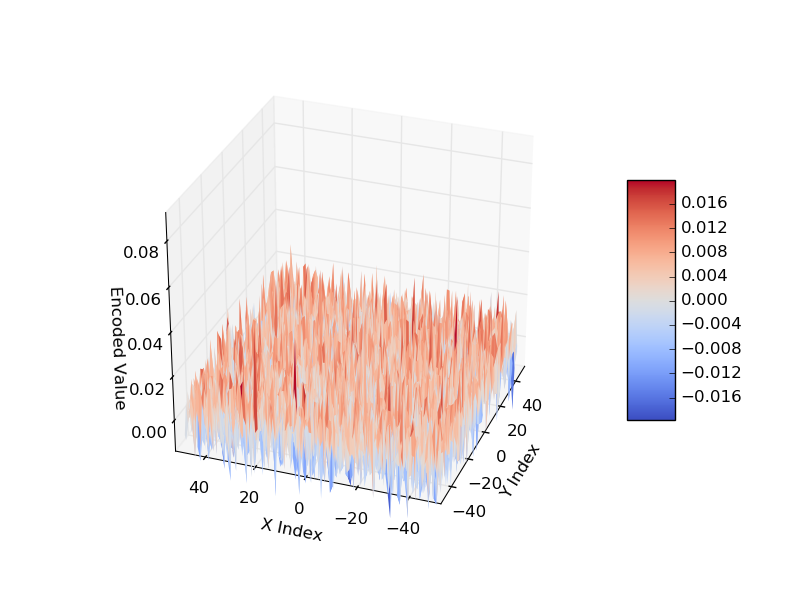
\includegraphics[width=\linewidth]{img/coord_example_2.png}
			\caption{Encoding of the "watch" object ID as a randomly sampled vector}
			\label{fig:encoding-object}
		\end{subfigure}
		
		\begin{subfigure}{0.8\columnwidth}
			\center
			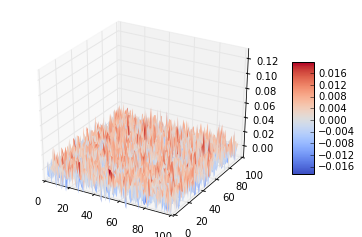
\includegraphics[width=0.8\linewidth]{img/coord_example_3.png}
			\caption{Representation of the complete visual scene, containing information about all 7 objects and their locations scrambled together}
			\label{fig:encoding-scene}
		\end{subfigure}
		
		\begin{subfigure}{0.45\columnwidth}
			\center
			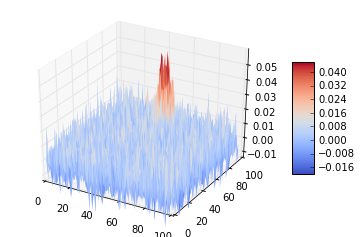
\includegraphics[width=\linewidth]{img/probe_for_mug.png}
			\caption{Probing for "mug" returns location probability for a mug}
			\label{fig:probing-single}
		\end{subfigure}
		\begin{subfigure}{0.45\columnwidth}
			\center
			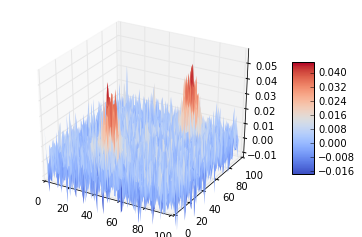
\includegraphics[width=\linewidth]{img/probe_for_pen.png}
			\caption{Probing for "pen" return mixture of Gaussian distributions}
			\label{fig:probing-double}
		\end{subfigure}
		
		\caption{Representation of visual scene in short term symbolic memory. }
		
	\end{figure}
	
	Due to the noisy nature of probing given by the slight loss of information in the binding process each symbol may have some amount of similarity to whatever other symbol it is compared to. However, even though this is the case, the similarity measure of bound symbols is consistently higher and can be clearly distinguished from others. Chart \ref{pgf:bar1} represents the result of probing at $(19, -26.75)$, which is somewhere in between the keys and the red pen, as seen in figure \ref{fig:object-detection}.
	
	 As we can see all symbols that are nowhere near the position present similarities well below $0.05$ (values may also be negative), while both close matches scored over $0.2$. Spot on probes may even attain values of over $0.5$. The example in chart \ref{pgf:bar2} is for a probe at $(-13, 21.5)$, which is further away from the center of an object region. But even though the dark pen and the wallet are further apart the result of probing still yields distinctly higher similarities for them as opposed to objects further away. 
	
	\begin{figure}[th!]
	\center
		\begin{subfigure}{0.49\columnwidth}
	    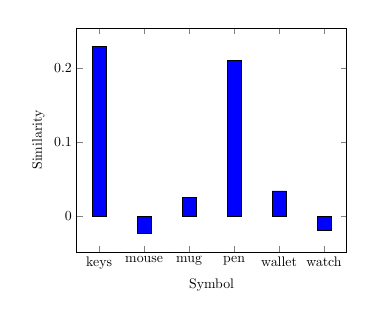
\begin{tikzpicture}[yscale=0.5, xscale=0.5]
        \begin{axis}[
            symbolic x coords={keys, mouse, mug, pen, wallet, watch},
            xlabel = Symbol,
            ylabel = Similarity
          ]
            \addplot[ybar,fill=blue] coordinates {
                (keys,   0.22827929349034107)
                (mouse, -0.023035819302988644)
                (mug, 0.025309361445942102)
                (pen, 0.2098596398998358)
                (wallet, 0.034187368731921304)
                (watch, -0.018549398363469777)
            };
        \end{axis}
    \end{tikzpicture}
        \caption{Probe at (19, -26.75).}
        \label{pgf:bar1}
    \end{subfigure}
		\begin{subfigure}{0.49\columnwidth}
    	    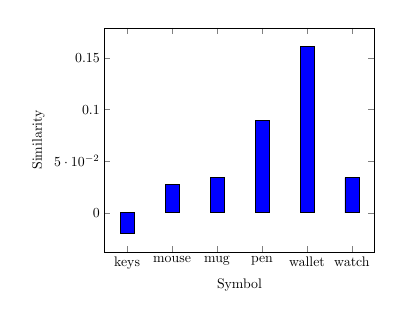
\begin{tikzpicture}[yscale=0.5, xscale=0.5]
        \begin{axis}[
            symbolic x coords={keys, mouse, mug, pen, wallet, watch},
            xlabel = Symbol,
            ylabel = Similarity
          ]
            \addplot[ybar,fill=blue] coordinates {
                (keys,   -0.020032173214673016)
                (mouse, 0.027742071303527464)
                (mug, 0.03443254630997427)
                (pen, 0.089801145874187763)
                (wallet, 0.16100011074269183)
                (watch, 0.034034204029029354)
            };
        \end{axis}
    \end{tikzpicture}	
        \caption{Probe at (-13, 21.5).}
        \label{pgf:bar2}
    \end{subfigure}
    
    			\caption{Similarity test for each symbol from the lookup table after probing the entire scene memory for a specific location.}
    \end{figure}

	

		\label{fig:visual-scene-exp}
	
\subsection{Symbolic scripting (holographic controllers)}

We have used our system to demonstrate a mechanism for encoding neural programs and processes through a series of associated action, perception and actuator symbols. We call this mechanism for defining controllers using holographic memories "symbolic scripting".


\begin{figure}[th!]
	\center
	\begin{subfigure}{1\columnwidth}
		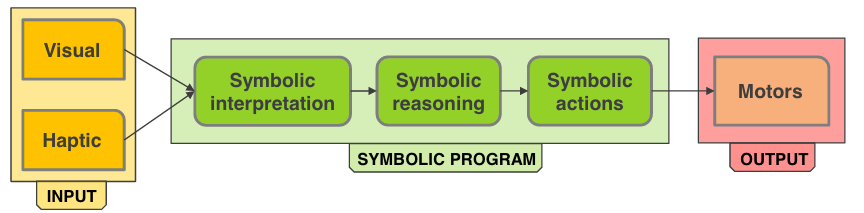
\includegraphics[width=\columnwidth]{img/control_pipeline.png}
		\caption{Symbolic scripting pipeline}
		\label{fig:symbolic-scripting-a}
	\end{subfigure}
	
	
	\begin{subfigure}{0.7\columnwidth}
		\center
		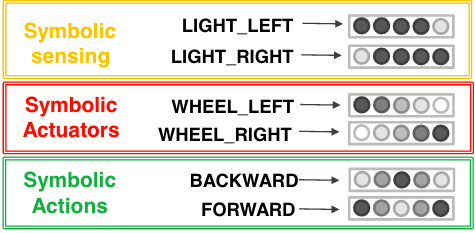
\includegraphics[width=\columnwidth]{img/symbol_table.png}
		\caption{Symbol table}
		\label{fig:symbolic-scripting-b}
	\end{subfigure}
	\begin{subfigure}{1\columnwidth}
		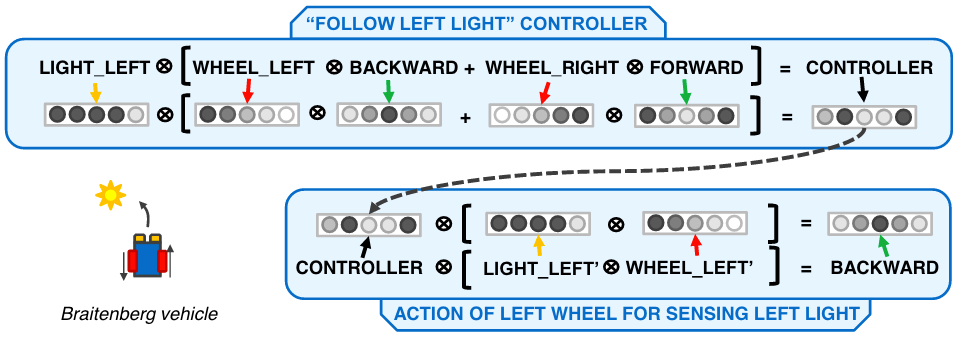
\includegraphics[width=\columnwidth]{img/controller.png}
		\caption{Holographic program (script)}
		\label{fig:symbolic-scripting-c}
	\end{subfigure}
	\caption{Symbolic scripting example for light following behavior of a two-wheeled robot}
	\label{fig:symbolic-scripting}
\end{figure}


The basic idea is centered around symbolic representations of all three parts involved:
\begin{enumerate}
	\item \textbf{actions} are symbolic constants representing groups of control signals, such as "forward", "backward", "stop", "flex", etc.
	
	\item \textbf{actuators} are named controllable parts of the system on which actions can be performed on, such as "right\_wheel", "left\_wheel", etc.
	
	\item \textbf{senses} are preprocessed (classified) sensory stream labels, such as "bright", "dark", "touching", "falling\_down", "rolling", etc.
\end{enumerate}

An example of this kind of symbolic script is given in figure \ref{fig:symbolic-scripting}. Here the memory encodes a light following behaviour.

		\begin{figure}[th!]
			\begin{subfigure}{0.45\columnwidth}
				\center
				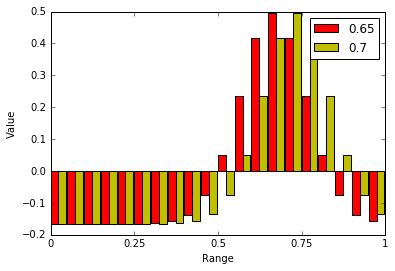
\includegraphics[width=1\columnwidth]{img/gaussianbar.png}
				\caption{Gaussian distribution without permutation.}
				\label{fig:gaussianbar}
			\end{subfigure}
			\begin{subfigure}{0.45\columnwidth}
				\center
				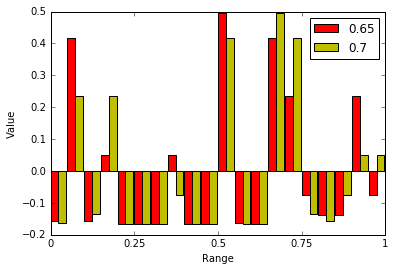
\includegraphics[width=1\columnwidth]{img/gaussianbarperm.png}
				\caption{Gaussian distribution with permutation.\\
				}
				\label{fig:gaussianbarperm}
			\end{subfigure}	
		\caption{Sensory input of an objects positions in the visual field at two points in time. A comparison between the raw generated input and its permuted version can be seen.}
		\label{gaussian}
		\end{figure}	

	\section{Conclusions}
	We have introduced a mechanism for intrinsic symbol encoding/decoding for Holographic Reduced Representations.
As a consequence, our approach eliminates the need for clean-up memories as they are described in literature.
Instead, results of probing operations directly give interpretable symbols, which can be decoded in constant computational time.
In other words, time needed for encoding/decoding is completely ignorant of the total number of symbols memorized, allowing memories that can store a large corpus of different symbols.
	A concrete biophysical evidence and theoretical model of implementation of convolution in the brain is, unfortunately, still missing.
	
	%% Add entry to the table of contents for the bibliography
	\printbibliography[heading=bibintoc]
	
	% that's all folks
\end{document}


